\documentclass[10pt]{article}

\pagestyle{plain}
\textwidth 6.5 in
\oddsidemargin 0 in
\evensidemargin 0 in
\topmargin 0 in
\textheight 8 in

\pagestyle{empty}

\usepackage[all]{xy}
\usepackage{graphicx}
\usepackage{units}
\usepackage{enumerate}
\usepackage[hidelinks]{hyperref}

\usepackage{amssymb, amsmath, pict2e}
 \pagestyle{myheadings}

\usepackage{pdfsync}
\usepackage{rotating}
\usepackage{multirow}
\usepackage[normalem]{ulem}
\usepackage{cancel}

\usepackage{color}
\usepackage[usenames,dvipsnames,svgnames,table]{xcolor}
\usepackage{pgf,tikz}
\usetikzlibrary{arrows}
\usepackage{environ}
\usepackage{environ}
\makeatletter
\newsavebox{\measure@tikzpicture}
\NewEnviron{scaletikzpicturetowidth}[1]{%
  \def\tikz@width{#1}%
  \def\tikzscale{1}\begin{lrbox}{\measure@tikzpicture}%
  \BODY
  \end{lrbox}%
  \pgfmathparse{#1/\wd\measure@tikzpicture}%
  \edef\tikzscale{\pgfmathresult}%
  \BODY
}


\title{Characterization and complexity of Thin Strip Graphs}

\author{Abdeselam El-Haman Abdeselam \\  Department of Computer Science \\ Universite Libre de Bruxelles}


\date{May 7, 2014}

%%%%%%%%%%%%%%%%  start macros  %%%%%%%%%%%%%%%%%%%%%%%%%%%%%%%%%
\newtheorem{theorem}{Theorem}
\newtheorem{defn}[theorem]{Definition}
\newtheorem{example}[theorem]{Example}
\newtheorem{remark}[theorem]{Remark}
\newtheorem{question}[theorem]{Question}

\newtheorem{lemma}[theorem]{Lemma}
\newtheorem{claim}[theorem]{Claim}
\newtheorem{prop}[theorem]{Proposition}
\newtheorem{corollary}[theorem]{Corollary}
\newtheorem{conjecture}[theorem]{Conjecture}

\newtheorem{hyp}[theorem]{Hypothesis}
\newtheorem{alg}[theorem]{Algorithm}

\newcommand{\qed}{\mbox{$\Box$}}
\newcommand{\proof}{\medbreak\par\noindent{\bf Proof. }}
 \newcommand{\GP}{{\vec{G}}_P}
\newcommand{\GN}{{\vec{G}}_N}

\newcommand{\cover}{\mathrel{\rlap{$\prec$}
                                \rlap{\hskip 0.7em $\cdot$}
                                 \phantom{\prec}}}

\newcommand{\re}{re}

\newcommand{\up}{\mbox{\rm{up}}}
\newcommand{\side}{\mbox{\rm{side}}}
\newcommand{\type}{\mbox{\rm{type}}}


\def\reals{{\mathbb R}}


\newcommand{\ahat}{{\hat{a}}}
\newcommand{\bhat}{{\hat{b}}}
\newcommand{\chat}{{\hat{c}}}
\newcommand{\dhat}{{\hat{d}}}
\newcommand{\bolda}{{\bf{a}}}
\newcommand{\boldb}{{\bf{b}}}
\newcommand{\boldc}{{\bf{c}}}
\newcommand{\boldd}{{\bf{d}}}

\newcommand{\iplus}{{\cal I}^+}
\newcommand{\iminus}{{\cal I}^-}
\newcommand{\ipm}{{\cal I}^{\pm}}
\newcommand{\ipmix}{{\cal I}^{{\cal M}}}

\newcommand{\upl}{{\cal U}^+}
\newcommand{\uminus}{{\cal U}^-}
\newcommand{\upm}{{\cal U}^{\pm}}
\newcommand{\upmix}{{\cal U}^{{\cal M}}}


\newcommand{\ppl}{{\cal P}^+}
\newcommand{\pminus}{{\cal P}^-}
\newcommand{\ppm}{{\cal P}^{\pm}}
\newcommand{\ppmix}{{\cal P}^{{\cal M}}}
\newcommand{\bpm}{{\cal B}^{\pm}}
\newcommand{\tpm}{{\cal T}^{\pm}}
\newcommand{\bpmix}{{\cal B}^{{\cal M}}}
\newcommand{\tpmix}{{\cal T}^{{\cal M}}}
%%%%%%%%%%%%%%%%  end macros  %%%%%%%%%%%%%%%%%%%%%%%%%%%%%%%%%

\begin{document}

  \maketitle

\bibliographystyle{plain}


\begin{center} {\sl ABSTRACT} \end{center}

\begin{quotation}

Abstract

\end{quotation}

%% This is an example first chapter.  You should put chapter/appendix that you
%% write into a separate file, and add a line \include{yourfilename} to
%% main.tex, where `yourfilename.tex' is the name of the chapter/appendix file.
%% You can process specific files by typing their names in at the
%% \files=
%% prompt when you run the file main.tex through LaTeX.
\section{Graphs and intersections}
\label{sec:graphs}


\subsection{Graphs}

A graph $G$ is defined as $G = (V,E)$, where $V$ is the set of vertices and $E$ the set of
edges, where $E \subseteq \binom{V}{2}$. The vertices $v,w \in V$ such that $e = vw \in E$
links are called the \textit{endpoints} of $e$.

\begin{defn}
  An embedding of a graph $G$ into a surface $\Sigma$ is a mapping of $G$ in
  $\Sigma$ where the vertices correspond to distinct points and the edges
  correspond to simple arcs connecting the images of their endpoints.
  \cite{goyalGraphEmbeddingTechniques2017}.
\end{defn}

A graph $G$ is planar if there is an embedding of this graph that does not have
any crossing between the edges.

\begin{defn}
  Let $G = (V,E)$ and $S \subset V$, an induced subgraph is a graph $H$ of $G$ whose
  vertex set is $S$ and its edge set $F = \{vw : v,w \in S, vw \in E\}$.
\end{defn}

\begin{defn}
  Let $G = (V,E)$ its complement graph $\overline{G}$ is the graph such that its edge set
  is defined as: $\{vw: v,w\in V, vw\notin E\}$.
\end{defn}

\begin{defn}
  $H$ is called a \textit{minor} of $G$ if $H$ can be constructed by deleting edges and vertices,
  or contracting edges.
\end{defn}

\begin{theorem}[Kuratowski]
  A graph $G$ is planar if and only if it does not contain $K_5$ or $K_{3,3}$ as a minor or
  a induced subgraph.
\end{theorem}

\begin{defn}
  A path $P_n$ in a graph $G$ is a sequence of vertices $v_1v_2v_3\dots v_n$ such
  that $v_iv_{i+1} \in E$.
\end{defn}

\begin{defn}
  A cycle $C_n$ in a graph $G = (V,E)$ is a path $v_1\dots v_n$ such that $v_1 = v_n$.
\end{defn}

\begin{defn}
  A chord of a cycle $C_n$ is an edge that connects two non consecutive vertices
  of $C_n$.
\end{defn}

\begin{defn}
  A graph $G = (V,E)$ is complete if every pair of distinct $v_1,v_2 \in V$ are
  adjacent. This is denoted $K_n$ with $n$ the size of the graph. If $G$ is an
  induced graph of $H$ then $G$ is a clique of $H$.
\end{defn}

\begin{defn}
  A graph $G$ is bipartite if there exist two disjoint subsets $A,B \subset V$ such
  that $A\cup B = V$ and each edge $e\in E$ has an endpoint on $A$ and the
  another on $B$.
\end{defn}

\begin{defn}
  A bipartite graph $G$ with bipartitions $A$ and $B$ is complete bipartite if
  every pair of vertices $v\in A, w\in B$ are adjacent. It is denoted as $K_{n,m}$,
  being $n$ and $m$ the size of each bipartition.
\end{defn}

\begin{defn}
  An induced forbidden subgraph of a graph class $X$ is a graph such that if it is the induced
  subgraph of a graph $G$, we know that $G \notin X$.
\end{defn}

The coloration of a graph is a color assignment to each vertex such that the color
of the two endpoints of every edge of the graph is different.

\begin{defn}
  The chromatic number of a graph $\chi(G)$ is the smallest number of colors needed to
  have an acceptable coloration of $G$.
\end{defn}

\begin{defn}
  The clique number of a graph $\omega(G)$ is the size of the biggest clique of $G$. We
  can observe that for every graph: $\chi(G) \geq \omega(G)$.
\end{defn}

\begin{defn}
  A perfect graph is a graph that respects this condition for every induced subgraph:
  $$ \omega(G) = \chi(G)$$
\end{defn}

\begin{theorem}[Lovasz]
  $G$ is perfect if and only if $\overline{G}$ is perfect.
\end{theorem}

\subsection{Intersection graphs}

\begin{defn}
The \textit{intersection graph} of a collection $\zeta$ of objects is the graph
$(\zeta,E)$ such that $c_1c_2\in E \Leftrightarrow c_1 \cap c_2 \neq \varnothing$.
\end{defn}


\begin{defn}
  A partial order set is a binary relation $\leq$ over a set $A$ satisfying these axioms:
  \begin{itemize}
    \item $a \leq a$ (reflexivity).
    \item if $a \leq b$ and $b \leq a$ then $a = b$ (antisymmetry).
    \item if $a \leq b$ and $b \leq c$ then $a \leq c$ (transitivity).
  \end{itemize}
\end{defn}

\begin{defn}
   A partially ordered set or poset  $(S,\leq)$ where $S$ a set and $\leq$ a partial
   order on $S$.
\end{defn}

\begin{defn}
  A graph $G = (V,E)$ is a comparibility graph if there exists a partial order
  $\leq$ such that $vw \in E \Leftrightarrow v \leq w$ or $w \leq v$.
  Equivalently, $G$ is a comparability graph if it is the comparability graph of
  a poset. For example, the Hasse diagram (figure \ref{fig:hasse}) is a
  comparability graph where the relation is inclusion.
\end{defn}

\begin{figure}
\centering

\begin{scaletikzpicturetowidth}{\textwidth}
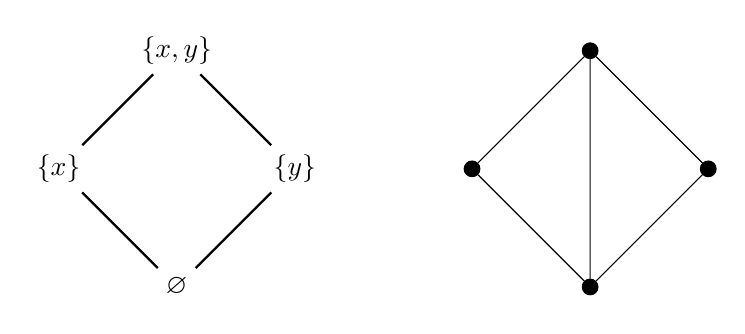
\begin{tikzpicture}[scale=1.5]

  % poset
  \draw (-1cm,0cm) node (v2) {$\{x\}$};
  \draw (1cm,0cm)  node (v3) { $\{y\}$ };
  \draw (0cm,-1cm) node (v4) {$\varnothing$};
  \draw (0cm,1cm)  node (v1) {$\{x,y\}$};

  \draw[thick]  (v1) edge (v2);
  \draw[thick]  (v3) edge (v1);
  \draw[thick]  (v3) edge (v4);
  \draw[thick]  (v2) edge (v4);

  % graph
  \node[draw,circle,inner sep=2pt,fill,label distance=1cm] (v1g) at (3.5,1) {};
  \node[draw,circle,inner sep=2pt,fill,label distance=1cm] (v2g) at (3.5,-1) {};
  \node[draw,circle,inner sep=2pt,fill,label distance=1cm] (v3g) at (4.5,0) {};
  \node[draw,circle,inner sep=2pt,fill,label distance=1cm] (v4g) at (2.5,0) {};
  \draw  (v1g) edge (v2g);
  \draw  (v1g) edge (v4g);
  \draw  (v4g) edge (v2g);
  \draw  (v1g) edge (v3g);
  \draw  (v3g) edge (v2g);

\end{tikzpicture}
\end{scaletikzpicturetowidth}

\caption{On the left, Hasse diagram of a poset of the power set of 2 elements ordered by inclusion.
On the right, the comparability graph of this poset.}
\label{fig:hasse}
\end{figure}

\subsubsection{Interval graphs}

An interval graph is a graph $G$ that is the intersection graph of a collection
of closed intervals in $\mathbb{R}$. If the length of each interval is unitary,
then $G$ is a unit interval graph (UIG).

\begin{theorem}
  $G$ is an interval graph if and only if every simple cycle of four or more
  points has a chord. \cite{FISHBURN1985135}
\end{theorem}

\begin{theorem}
  An interval graph is a unit interval graph if and only if it has no induced subgraph $K_{1,3}$ \cite{roberts1968representations}.
\end{theorem}

Another interesting class of interval graphs are mixed unit interval graphs, where each
interval can be closed, open, open-closed or closed-open. In this paper we will
denote those four classes like this:

$$\mathcal{I}^{++} = \{[x,y] : x,y \in \mathbb{R}, x\leq y\}$$
$$\mathcal{I}^{--} = \{(x,y) : x,y \in \mathbb{R}, x\leq y\}$$
$$\mathcal{I}^{+-} = \{[x,y) : x,y \in \mathbb{R}, x\leq y\}$$
$$\mathcal{I}^{-+} = \{(x,y] : x,y \in \mathbb{R}, x\leq y\}$$

$\mathcal{I}$ will be replaced by $\mathcal{U}$ when we are talking about unit
mixed interval graphs and their class is denoted MUIG.

\begin{theorem}
  The classes of the graphs $\mathcal{U}^{--}$, $\mathcal{U}^{++}$,
  $\mathcal{U}^{-+}$, $\mathcal{U}^{+-}$, and  $\mathcal{U}^{-+} \cup
  \mathcal{U}^{+-}$ are the same (equivalent for $\mathcal{I}$). \cite{DOURADO20123357}
\end{theorem}



\begin{figure}
\centering


\begin{scaletikzpicturetowidth}{\textwidth}
\begin{tikzpicture}[scale=1.5]

  \draw[{(-)}] (-1,-0.5) -- (0,-0.5);
  \draw[color=black] (-0.4845,-0.8507) node {$v_4$};
  \draw[{[-}] (0,-1.5) -- (1,-1.5);
  \draw[color=black] (0.5023,-1.3568) node {$v_3$};
  \draw[{-]}] (-2,-1.5) -- (-1,-1.5);
  \draw[color=black] (-0.4899,-0.3468) node {$v_2$};
  \draw[{[-]}] (-1,-1) -- (0,-1);
  \draw[color=black] (-1.4962,-1.3536) node {$v_1$};

  \node[draw,circle,inner sep=2pt,fill,label distance=1cm] (v1) at (-4,-0.25) {};
  \draw[color=black] (-4,0) node {$v_4$};
  \node[draw,circle,inner sep=2pt,fill,label distance=1cm] (v3) at (-4,-1.25) {};
  \draw[color=black] (-4,-1.5) node {$v_2$};
  \node[draw,circle,inner sep=2pt,fill,label distance=1cm] (v2) at (-5,-1.25) {};
  \draw[color=black] (-3,-1.5) node {$v_3$};
  \node[draw,circle,inner sep=2pt,fill,label distance=1cm] (v4) at (-3,-1.25) {};
  \draw[color=black] (-5,-1.5) node {$v_1$};
  \draw  (v1) edge (v2);
  \draw  (v1) edge (v3);
  \draw  (v1) edge (v4);

\end{tikzpicture}
\end{scaletikzpicturetowidth}

\caption{Representation of $K_{1,3}$ as a MUIG.}
\label{fig:muigK13}
\end{figure}

Unlike for UIG class, $K_{1,3}$ is a MUIG as seen in figure \ref{fig:muigK13}. Some
characterizations have been already found for these classes of graphs \cite{shuchatUnitMixedInterval2014}
\cite{joosCharacterizationMixedUnit2013}.

\subsubsection{Disks}

A disk graph $G$ is a graph that is an intersection graph of disks on the plane, when the size
of the disk is unitary, we talk about unit disk graphs. This class of graphs
is important for this thesis, as thin strip graphs are a sub-class of
unit disk graphs (section \ref{sec:thin}).

We will refer to the unit disk graph class as UDG and an example of a realization
can be found in the figure \ref{fig:udg}.

\paragraph{Induced forbidden subgraphs} The characterization of this class with respect to
its induced forbidden subgraphs have been studied \cite{atminasForbiddenInducedSubgraphs2016}.

\begin{theorem}[Atminas-Zamaraev]
  For every integer $k > 1$, $\overline{K_2 + C_{2k+1}}$ is a minimal induced subgraph.
\end{theorem}

\begin{theorem}[Atminas-Zamaraev]
  For every integer $k > 4$, $\overline{C_{2k}}$ is a minimal induced subgraph.
\end{theorem}

\begin{figure}
\centering

\begin{scaletikzpicturetowidth}{\textwidth}
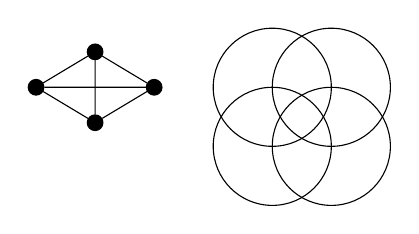
\begin{tikzpicture}[scale=1.5]

  \draw (-0.5,2.5) circle [radius=0.5];
  \draw (0,2.5) circle [radius=0.5];
  \draw (-0.5,2) circle [radius=0.5];
  \draw (0,2) circle [radius=0.5];


  \node[draw,circle,inner sep=2pt,fill,label distance=1cm] (v1) at (-2.5,2.5) {};

  \node[draw,circle,inner sep=2pt,fill,label distance=1cm] (v2) at (-2,2.2) {};
  \node[draw,circle,inner sep=2pt,fill,label distance=1cm] (v3) at (-2,2.8) {};
  \node[draw,circle,inner sep=2pt,fill,label distance=1cm] (v4) at (-1.5,2.5) {};

  \draw  (v3) edge (v2);
  \draw  (v4) edge (v1);
  \draw  (v3) edge (v1);
  \draw  (v4) edge (v2);
  \draw  (v3) edge (v4);
  \draw  (v1) edge (v2);

\end{tikzpicture}
\end{scaletikzpicturetowidth}

\caption{Realization of a UDG (Unit Disk Graph).}
\label{fig:udg}
\end{figure}

%% This is an example first chapter.  You should put chapter/appendix that you
%% write into a separate file, and add a line \include{yourfilename} to
%% main.tex, where `yourfilename.tex' is the name of the chapter/appendix file.
%% You can process specific files by typing their names in at the
%% \files=
%% prompt when you run the file main.tex through LaTeX.
\section{Complexity}

Problem solving is based on the complexity of a problem and not only a particular algorithm that solves it \cite{sipser2006}.

\begin{defn}
Let $\Sigma$ be a finite alphabet, $\Sigma^*$ every word derived from $\Sigma$, $L \subseteq \Sigma^*$ is a decision problem.
\end{defn}

\begin{defn}
The algorithm $A$ decides problem $L \subseteq \Sigma^*$ if for all word $w \in \Sigma^*$:
\begin{itemize}
  \item $A$ finishes and returns TRUE if $w \in L$.
  \item $A$ finishes and returns FALSE if $w \notin L$.
\end{itemize}
\end{defn}

\begin{defn}
A problem is decidable if there's an algorithm that decides it.
\end{defn}

\begin{defn}
A problem is decidable if there's an algorithm that decides it.
\end{defn}

\subsection{P vs NP}

\begin{defn}
A problem $L \in \mathcal{P}$ if $L$ can be decided in polynomial time $\mathcal{O}(n^k)$.
\end{defn}

\begin{defn}
A problem $L \in \mathcal{NP}$ if $L$ can be verified in polynomial time $\mathcal{O}(n^k)$. Thus, $\mathcal{P} \subseteq \mathcal{NP}$.
\end{defn}

\subsection{$\exists \mathbb{R}$ complexity class}

$\exists \mathbb{R}$ is the class that describes the problems such that they can be reduced to \textit{the existential theory of the reals}\cite{ExistentialTheoryReals2006}. The existential theory of the reals

\subsubsection{Problems in $\exists \mathbb{R}$}

The art gallery problem is $\exists \mathbb{R}$-complete.\cite{abrahamsenArtGalleryProblem2017}

Recognition of Unit Disk Graphs is $\exists \mathbb{R}$-complete. (corollary of graph realizability problem)\cite{Schaefer2013}

Stretchability is $\exists \mathbb{R}$-complete.

%% This is an example first chapter.  You should put chapter/appendix that you
%% write into a separate file, and add a line \include{yourfilename} to
%% main.tex, where `yourfilename.tex' is the name of the chapter/appendix file.
%% You can process specific files by typing their names in at the
%% \files=
%% prompt when you run the file main.tex through LaTeX.
\section{Geometry}
\label{sec:geom}

\subsection{Stabbing}

Definition of stabbing.

Stabbing geometric structures.\cite{schlipf2013stabbing}

Koebe's planar $\subseteq$ disk
  = Planar graph duality

Helly's theorem

%% This is an example first chapter.  You should put chapter/appendix that you
%% write into a separate file, and add a line \include{yourfilename} to
%% main.tex, where `yourfilename.tex' is the name of the chapter/appendix file.
%% You can process specific files by typing their names in at the
%% \files=
%% prompt when you run the file main.tex through LaTeX.
\section{Disk Graph studies}

\subsection{Stabbing disks}

Definition of stabbing.

Stabbing geometric structures.\cite{schlipf2013stabbing}

\subsection{Thin Strip Graphs}

$c$-strip graphs are unit disk graphs such that the centers of the disks are delimited on the area $\{(x,y) : -\infty < x < \infty, 0 < y \leq c\}$ and its class noted SG($c$). We can say that SG(0) = UIG and SG($\infty$) = UDG. \cite{hayashiThinStripGraphs2017}

\begin{defn}
  Thin strip graphs are defined as TSG $= \bigcap_{c > 0}$ SG($c$).
\end{defn}

\begin{remark}
  SG($0$) $\neq$ TSG. This can be seen
\end{remark}

\begin{figure}
\centering
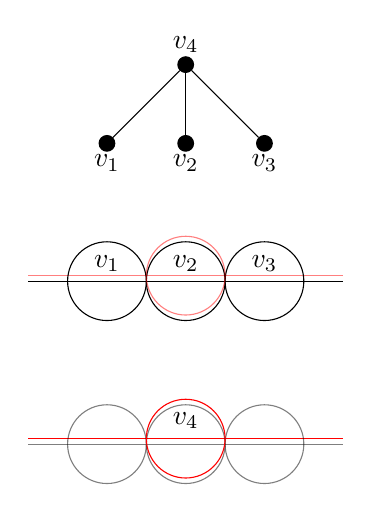
\begin{tikzpicture}
\draw (-2,0) -- (2,0);
\draw[red ,opacity = 0.5] (-2,0.07) -- (2,0.07);
\draw  (-1,0) circle [radius=0.5];
\draw[color=black] (-1,0.2265) node {$v_1$};
\draw  (0,0) circle [radius=0.5];
\draw[color=black] (0,0.2265) node {$v_2$};
\draw  (1,0) circle [radius=0.5];
\draw[color=black] (1,0.2265) node {$v_3$};

\draw[red, opacity = 0.5] (0,0.07) circle [radius=0.5];

\draw[opacity = 0.5] (-2,-2.07) -- (2,-2.07);
\draw[red] (-2,-2) -- (2,-2);
\draw[opacity = 0.5]  (0,-2.07) circle [radius=0.5];
\draw[opacity = 0.5]  (1,-2.07) circle [radius=0.5];
\draw[opacity = 0.5]  (-1,-2.07) circle [radius=0.5];
\draw[red] (0,-2) circle [radius=0.5];
\draw[color=black] (0,-1.765) node {$v_4$};

\node[draw,circle,inner sep=2pt,fill,label distance=1cm] (v1) at (0,2.75) {};
\draw[color=black] (0,3) node {$v_4$};
\node[draw,circle,inner sep=2pt,fill,label distance=1cm] (v3) at (0,1.75) {};
\draw[color=black] (0,1.5) node {$v_2$};
\node[draw,circle,inner sep=2pt,fill,label distance=1cm] (v2) at (-1,1.75) {};
\draw[color=black] (1,1.5) node {$v_3$};
\node[draw,circle,inner sep=2pt,fill,label distance=1cm] (v4) at (1,1.75) {};
\draw[color=black] (-1,1.5) node {$v_1$};
\draw  (v1) edge (v2);
\draw  (v1) edge (v3);
\draw  (v1) edge (v4);
\end{tikzpicture}
\end{figure}

$K_{1,3}$ in TSG, which is not possible for UIG.

MUIG $\subsetneq$ TSG.\\


Denote that there's not constant $t$ such that SG($t$) = TSG.\\

Unfettered unit interval graphs = UUIG\\

MUIG $\subsetneq$ TSG $\subsetneq$ UUIG

\begin{defn}
  Find forbidden induced graphs for TSG.
\end{defn}


\bibliography{main}

\end{document}
